% Informe del laboratorio 6: control discreto en el PLC y middleware de telemetría
% Compilar desde esta carpeta: pdflatex informe_lab06.tex (dos veces)
\documentclass[a4paper,11pt]{article}
% Preámbulo común de los informes de laboratorio (II/2026). Se incluye desde laboratorios/labNN_*/
%   % Preámbulo común de los informes de laboratorio (II/2026). Se incluye desde laboratorios/labNN_*/
%   % Preámbulo común de los informes de laboratorio (II/2026). Se incluye desde laboratorios/labNN_*/
%   \input{../informe_comun}
\input{../../gemelo-digital/manual/estilo_manual}
\input{../../gemelo-digital/manual/tecnico/macros}
\graphicspath{{../../documentacion/planos_isa/pid/}{../../documentacion/planos_isa/electrico/}{../../documentacion/manuales_inversa/}
  {../../database/mockups/}{../../database/documentacion/}{../../database/modelo/}{../../database/interfaz/}
  {../../gemelo-digital/manual/img/}{../../modelo-3d/informe/figuras/}{../../modelo-3d/levantamiento/}{../../../../global/fotos-planta/}{../figuras/}}
\usepackage{pdflscape}
\lstset{showstringspaces=false}
% plano A3 en una página apaisada: \plano[página]{archivo}{leyenda}
\newcommand{\plano}[3][1]{\begin{landscape}\begin{figure}[p]\centering\includegraphics[page=#1, width=\linewidth, height=0.86\textwidth, keepaspectratio]{#2}\caption{#3}\end{figure}\end{landscape}}
\setlength{\headheight}{14pt}
\newcommand{\nlab}{}
\newcommand{\tlab}{}
\lhead{\small Brazo XK-JS1-1 · Informe del laboratorio \nlab}
\rhead{\small UMSA · II/2026}

% \portada{número}{título}{inicio}{entrega}{semanas}
\newcommand{\portada}[5]{%
\renewcommand{\nlab}{#1}%
\begin{titlepage}
\centering
\vspace*{0.6cm}
{\large Universidad Mayor de San Andrés · Facultad de Ingeniería\par}
{\large Carrera de Ingeniería Electrónica\par}
\vspace{0.8cm}
{\color{naranja!80!black}\rule{\linewidth}{1.5pt}\par}
\vspace{0.3cm}
{\Large Informe del Laboratorio Integrado Nº #1\par}
\vspace{0.2cm}
{\huge\bfseries #2\par}
\vspace{0.3cm}
{\color{naranja!80!black}\rule{\linewidth}{1.5pt}\par}
\vspace{0.8cm}
{\large Planta: brazo robótico XK-JS1-1 de 4 grados de libertad\par}
\vspace{0.3cm}
{\large ETN-902 Sistemas de Control II · ETN-1034 Aplicación de Técnicas de Control · ETN-1000 Bases de Datos\par}
\vspace{1cm}
\begin{tabular}{rl}
\textbf{Docente:} & Ing. Jorge Antonio Nava Amador\\
\textbf{Auxiliares:} & Limber Ajnota · Fabián Plata · Franz Choque\\
\textbf{Inicio de trabajo:} & #3\\
\textbf{Entrega:} & #4 (#5)\\
\end{tabular}
\vspace{1cm}

\begin{tabular}{ll}
\multicolumn{2}{l}{\textbf{Escuadra del brazo de 4 GDL}}\\[2pt]
Control (ETN-902 / ETN-1034): & Gabriel Andres Gomez Calla\\
 & Jose Lenin Mamani Choque\\
 & Miguel Alejandro Lima Huarachi\\
 & Román Abner Machicado Arequipa\\[2pt]
Cómputo (ETN-1000): & Miguel Alejandro Lima Huarachi\\
 & Marco Eduardo Chura Rondo\\
\end{tabular}
\vfill
{\small Repositorio: \url{https://github.com/GabAndGom/Brazo-de-4-grados-de-libertad}\par}
{\small La Paz, Bolivia · gestión II/2026\par}
\end{titlepage}
}

% Tabla de entregables (Definition of Done): \begin{dod} ... \end{dod}, filas: entregable & estado & evidencia\\
\newenvironment{dod}{\begin{center}\small\begin{longtable}{>{\raggedright}p{5.2cm} >{\raggedright}p{1.8cm} >{\raggedright\arraybackslash}p{7.6cm}}
\toprule \textbf{Entregable} & \textbf{Estado} & \textbf{Evidencia / observación}\\ \midrule \endhead}
{\bottomrule\end{longtable}\end{center}}

\input{../../gemelo-digital/manual/estilo_manual}
% Macros del manual técnico: ladder, estados, código y rutas de imágenes
\usetikzlibrary{shapes.multipart}
\graphicspath{{../img/}{../../../../../global/fotos-planta/}{../../../modelo-3d/informe/figuras/}{../../../modelo-3d/levantamiento/}{../../../database/modelo/}{../../../documentacion/manuales_inversa/}{../../../documentacion/planos_isa/electrico/}{../../../database/interfaz/}}

\lstdefinestyle{py}{language=Python, keywordstyle=\color{azulg}\bfseries, commentstyle=\color{grisos}\itshape,
  stringstyle=\color{verde}, basicstyle=\ttfamily\scriptsize, numbers=left, numberstyle=\tiny\color{grisos}}
\lstdefinestyle{js}{language=Java, morekeywords={const,let,function,async,await,return,for,of,if,else}, keywordstyle=\color{azulg}\bfseries,
  commentstyle=\color{grisos}\itshape, stringstyle=\color{verde}, basicstyle=\ttfamily\scriptsize, numbers=left, numberstyle=\tiny\color{grisos}}
\lstdefinestyle{awl}{basicstyle=\ttfamily\tiny, commentstyle=\color{grisos}\itshape, morecomment=[l]{//},
  keywordstyle=\color{azulg}\bfseries, morekeywords={LD,LDN,A,AN,O,ON,EU,ED,S,R,MOVB,MOVW,MOVD,PLS,TON,CALL,CRET,LPS,LRD,LPP,ALD,OLD,FILL,LDW,LDB,LDD,AW,AD,AB,OW,OD},
  numbers=left, numberstyle=\tiny\color{grisos}, frame=single, backgroundcolor=\color{gris}}
\lstdefinestyle{sql}{language=SQL, keywordstyle=\color{azulg}\bfseries, commentstyle=\color{grisos}\itshape,
  stringstyle=\color{verde}, basicstyle=\ttfamily\tiny, numbers=left, numberstyle=\tiny\color{grisos},
  morekeywords={REFERENCES,SERIAL,SMALLSERIAL,BIGSERIAL,TIMESTAMPTZ,BOOLEAN,INET,RETURNS,TRIGGER,LANGUAGE,DECLARE,RAISE,EXCEPTION,VIEW,INDEX}}

\tikzset{
  ld/.style={line width=0.7pt},
  pics/na/.style={code={\fill[white](-0.12,-0.26) rectangle (0.12,0.26);
     \draw[thick](-0.1,-0.24)--(-0.1,0.24)(0.1,-0.24)--(0.1,0.24);
     \node[font=\scriptsize\ttfamily, above] at (0,0.22){#1};}},
  pics/nc/.style={code={\fill[white](-0.12,-0.26) rectangle (0.12,0.26);
     \draw[thick](-0.1,-0.24)--(-0.1,0.24)(0.1,-0.24)--(0.1,0.24);\draw(-0.17,-0.24)--(0.17,0.24);
     \node[font=\scriptsize\ttfamily, above] at (0,0.22){#1};}},
  pics/pf/.style={code={\fill[white](-0.12,-0.26) rectangle (0.12,0.26);
     \draw[thick](-0.1,-0.24)--(-0.1,0.24)(0.1,-0.24)--(0.1,0.24);
     \node[font=\tiny\bfseries] at (0,0){P};}},
  pics/cmp/.style n args={3}{code={\fill[white](-0.12,-0.26) rectangle (0.12,0.26);
     \draw[thick](-0.1,-0.24)--(-0.1,0.24)(0.1,-0.24)--(0.1,0.24);
     \node[font=\tiny\ttfamily] at (0,0){#2};
     \node[font=\scriptsize\ttfamily, above] at (0,0.22){#1};
     \node[font=\scriptsize\ttfamily, below] at (0,-0.22){#3};}},
  pics/bob/.style n args={3}{code={\fill[white](-0.2,-0.26) rectangle (0.2,0.26);
     \draw[thick](-0.05,0.24) arc (110:250:0.255);\draw[thick](0.05,0.24) arc (70:-70:0.255);
     \node[font=\tiny\bfseries] at (0,0){#2};
     \node[font=\scriptsize\ttfamily, above] at (0,0.22){#1};
     \node[font=\scriptsize\ttfamily, below] at (0,-0.22){#3};}},
  fb/.style={draw, fill=white, font=\scriptsize\ttfamily, align=left, inner sep=3pt, anchor=west},
  barra/.style={line width=2pt},
  estado/.style={draw, rounded corners=3pt, fill=white, align=center, font=\scriptsize, minimum width=22mm, minimum height=10mm, inner sep=3pt},
  estadon/.style={estado, fill=naranja!14, draw=naranja!70!black},
  trans/.style={font=\scriptsize, align=center, fill=white, inner sep=1pt},
  lugar/.style={circle, draw, thick, minimum size=7mm, fill=white},
  transicion/.style={rectangle, fill=black, minimum width=1.6mm, minimum height=7mm, inner sep=0},
  tabla/.style={rectangle split, rectangle split parts=2, draw, fill=white, font=\tiny\ttfamily, align=left, inner sep=2pt, rounded corners=1pt, text width=33mm},
}
\newcommand{\pendiente}[1]{\par\smallskip\noindent\colorbox{naranja!12}{\parbox{\dimexpr\linewidth-2\fboxsep}{\textbf{\color{naranja!80!black}Pendiente.} #1}}\par\smallskip}
\newcommand{\cumple}{\textcolor{verde}{\textbf{cumplido}}}
\newcommand{\parcial}{\textcolor{naranja}{\textbf{parcial}}}
\newcommand{\falta}{\textcolor{rojo}{\textbf{pendiente}}}

\graphicspath{{../../documentacion/planos_isa/pid/}{../../documentacion/planos_isa/electrico/}{../../documentacion/manuales_inversa/}
  {../../database/mockups/}{../../database/documentacion/}{../../database/modelo/}{../../database/interfaz/}
  {../../gemelo-digital/manual/img/}{../../modelo-3d/informe/figuras/}{../../modelo-3d/levantamiento/}{../../../../global/fotos-planta/}{../figuras/}}
\usepackage{pdflscape}
\lstset{showstringspaces=false}
% plano A3 en una página apaisada: \plano[página]{archivo}{leyenda}
\newcommand{\plano}[3][1]{\begin{landscape}\begin{figure}[p]\centering\includegraphics[page=#1, width=\linewidth, height=0.86\textwidth, keepaspectratio]{#2}\caption{#3}\end{figure}\end{landscape}}
\setlength{\headheight}{14pt}
\newcommand{\nlab}{}
\newcommand{\tlab}{}
\lhead{\small Brazo XK-JS1-1 · Informe del laboratorio \nlab}
\rhead{\small UMSA · II/2026}

% \portada{número}{título}{inicio}{entrega}{semanas}
\newcommand{\portada}[5]{%
\renewcommand{\nlab}{#1}%
\begin{titlepage}
\centering
\vspace*{0.6cm}
{\large Universidad Mayor de San Andrés · Facultad de Ingeniería\par}
{\large Carrera de Ingeniería Electrónica\par}
\vspace{0.8cm}
{\color{naranja!80!black}\rule{\linewidth}{1.5pt}\par}
\vspace{0.3cm}
{\Large Informe del Laboratorio Integrado Nº #1\par}
\vspace{0.2cm}
{\huge\bfseries #2\par}
\vspace{0.3cm}
{\color{naranja!80!black}\rule{\linewidth}{1.5pt}\par}
\vspace{0.8cm}
{\large Planta: brazo robótico XK-JS1-1 de 4 grados de libertad\par}
\vspace{0.3cm}
{\large ETN-902 Sistemas de Control II · ETN-1034 Aplicación de Técnicas de Control · ETN-1000 Bases de Datos\par}
\vspace{1cm}
\begin{tabular}{rl}
\textbf{Docente:} & Ing. Jorge Antonio Nava Amador\\
\textbf{Auxiliares:} & Limber Ajnota · Fabián Plata · Franz Choque\\
\textbf{Inicio de trabajo:} & #3\\
\textbf{Entrega:} & #4 (#5)\\
\end{tabular}
\vspace{1cm}

\begin{tabular}{ll}
\multicolumn{2}{l}{\textbf{Escuadra del brazo de 4 GDL}}\\[2pt]
Control (ETN-902 / ETN-1034): & Gabriel Andres Gomez Calla\\
 & Jose Lenin Mamani Choque\\
 & Miguel Alejandro Lima Huarachi\\
 & Román Abner Machicado Arequipa\\[2pt]
Cómputo (ETN-1000): & Miguel Alejandro Lima Huarachi\\
 & Marco Eduardo Chura Rondo\\
\end{tabular}
\vfill
{\small Repositorio: \url{https://github.com/GabAndGom/Brazo-de-4-grados-de-libertad}\par}
{\small La Paz, Bolivia · gestión II/2026\par}
\end{titlepage}
}

% Tabla de entregables (Definition of Done): \begin{dod} ... \end{dod}, filas: entregable & estado & evidencia\\
\newenvironment{dod}{\begin{center}\small\begin{longtable}{>{\raggedright}p{5.2cm} >{\raggedright}p{1.8cm} >{\raggedright\arraybackslash}p{7.6cm}}
\toprule \textbf{Entregable} & \textbf{Estado} & \textbf{Evidencia / observación}\\ \midrule \endhead}
{\bottomrule\end{longtable}\end{center}}

\input{../../gemelo-digital/manual/estilo_manual}
% Macros del manual técnico: ladder, estados, código y rutas de imágenes
\usetikzlibrary{shapes.multipart}
\graphicspath{{../img/}{../../../../../global/fotos-planta/}{../../../modelo-3d/informe/figuras/}{../../../modelo-3d/levantamiento/}{../../../database/modelo/}{../../../documentacion/manuales_inversa/}{../../../documentacion/planos_isa/electrico/}{../../../database/interfaz/}}

\lstdefinestyle{py}{language=Python, keywordstyle=\color{azulg}\bfseries, commentstyle=\color{grisos}\itshape,
  stringstyle=\color{verde}, basicstyle=\ttfamily\scriptsize, numbers=left, numberstyle=\tiny\color{grisos}}
\lstdefinestyle{js}{language=Java, morekeywords={const,let,function,async,await,return,for,of,if,else}, keywordstyle=\color{azulg}\bfseries,
  commentstyle=\color{grisos}\itshape, stringstyle=\color{verde}, basicstyle=\ttfamily\scriptsize, numbers=left, numberstyle=\tiny\color{grisos}}
\lstdefinestyle{awl}{basicstyle=\ttfamily\tiny, commentstyle=\color{grisos}\itshape, morecomment=[l]{//},
  keywordstyle=\color{azulg}\bfseries, morekeywords={LD,LDN,A,AN,O,ON,EU,ED,S,R,MOVB,MOVW,MOVD,PLS,TON,CALL,CRET,LPS,LRD,LPP,ALD,OLD,FILL,LDW,LDB,LDD,AW,AD,AB,OW,OD},
  numbers=left, numberstyle=\tiny\color{grisos}, frame=single, backgroundcolor=\color{gris}}
\lstdefinestyle{sql}{language=SQL, keywordstyle=\color{azulg}\bfseries, commentstyle=\color{grisos}\itshape,
  stringstyle=\color{verde}, basicstyle=\ttfamily\tiny, numbers=left, numberstyle=\tiny\color{grisos},
  morekeywords={REFERENCES,SERIAL,SMALLSERIAL,BIGSERIAL,TIMESTAMPTZ,BOOLEAN,INET,RETURNS,TRIGGER,LANGUAGE,DECLARE,RAISE,EXCEPTION,VIEW,INDEX}}

\tikzset{
  ld/.style={line width=0.7pt},
  pics/na/.style={code={\fill[white](-0.12,-0.26) rectangle (0.12,0.26);
     \draw[thick](-0.1,-0.24)--(-0.1,0.24)(0.1,-0.24)--(0.1,0.24);
     \node[font=\scriptsize\ttfamily, above] at (0,0.22){#1};}},
  pics/nc/.style={code={\fill[white](-0.12,-0.26) rectangle (0.12,0.26);
     \draw[thick](-0.1,-0.24)--(-0.1,0.24)(0.1,-0.24)--(0.1,0.24);\draw(-0.17,-0.24)--(0.17,0.24);
     \node[font=\scriptsize\ttfamily, above] at (0,0.22){#1};}},
  pics/pf/.style={code={\fill[white](-0.12,-0.26) rectangle (0.12,0.26);
     \draw[thick](-0.1,-0.24)--(-0.1,0.24)(0.1,-0.24)--(0.1,0.24);
     \node[font=\tiny\bfseries] at (0,0){P};}},
  pics/cmp/.style n args={3}{code={\fill[white](-0.12,-0.26) rectangle (0.12,0.26);
     \draw[thick](-0.1,-0.24)--(-0.1,0.24)(0.1,-0.24)--(0.1,0.24);
     \node[font=\tiny\ttfamily] at (0,0){#2};
     \node[font=\scriptsize\ttfamily, above] at (0,0.22){#1};
     \node[font=\scriptsize\ttfamily, below] at (0,-0.22){#3};}},
  pics/bob/.style n args={3}{code={\fill[white](-0.2,-0.26) rectangle (0.2,0.26);
     \draw[thick](-0.05,0.24) arc (110:250:0.255);\draw[thick](0.05,0.24) arc (70:-70:0.255);
     \node[font=\tiny\bfseries] at (0,0){#2};
     \node[font=\scriptsize\ttfamily, above] at (0,0.22){#1};
     \node[font=\scriptsize\ttfamily, below] at (0,-0.22){#3};}},
  fb/.style={draw, fill=white, font=\scriptsize\ttfamily, align=left, inner sep=3pt, anchor=west},
  barra/.style={line width=2pt},
  estado/.style={draw, rounded corners=3pt, fill=white, align=center, font=\scriptsize, minimum width=22mm, minimum height=10mm, inner sep=3pt},
  estadon/.style={estado, fill=naranja!14, draw=naranja!70!black},
  trans/.style={font=\scriptsize, align=center, fill=white, inner sep=1pt},
  lugar/.style={circle, draw, thick, minimum size=7mm, fill=white},
  transicion/.style={rectangle, fill=black, minimum width=1.6mm, minimum height=7mm, inner sep=0},
  tabla/.style={rectangle split, rectangle split parts=2, draw, fill=white, font=\tiny\ttfamily, align=left, inner sep=2pt, rounded corners=1pt, text width=33mm},
}
\newcommand{\pendiente}[1]{\par\smallskip\noindent\colorbox{naranja!12}{\parbox{\dimexpr\linewidth-2\fboxsep}{\textbf{\color{naranja!80!black}Pendiente.} #1}}\par\smallskip}
\newcommand{\cumple}{\textcolor{verde}{\textbf{cumplido}}}
\newcommand{\parcial}{\textcolor{naranja}{\textbf{parcial}}}
\newcommand{\falta}{\textcolor{rojo}{\textbf{pendiente}}}

\graphicspath{{../../documentacion/planos_isa/pid/}{../../documentacion/planos_isa/electrico/}{../../documentacion/manuales_inversa/}
  {../../database/mockups/}{../../database/documentacion/}{../../database/modelo/}{../../database/interfaz/}
  {../../gemelo-digital/manual/img/}{../../modelo-3d/informe/figuras/}{../../modelo-3d/levantamiento/}{../../../../global/fotos-planta/}{../figuras/}}
\usepackage{pdflscape}
\lstset{showstringspaces=false}
% plano A3 en una página apaisada: \plano[página]{archivo}{leyenda}
\newcommand{\plano}[3][1]{\begin{landscape}\begin{figure}[p]\centering\includegraphics[page=#1, width=\linewidth, height=0.86\textwidth, keepaspectratio]{#2}\caption{#3}\end{figure}\end{landscape}}
\setlength{\headheight}{14pt}
\newcommand{\nlab}{}
\newcommand{\tlab}{}
\lhead{\small Brazo XK-JS1-1 · Informe del laboratorio \nlab}
\rhead{\small UMSA · II/2026}

% \portada{número}{título}{inicio}{entrega}{semanas}
\newcommand{\portada}[5]{%
\renewcommand{\nlab}{#1}%
\begin{titlepage}
\centering
\vspace*{0.6cm}
{\large Universidad Mayor de San Andrés · Facultad de Ingeniería\par}
{\large Carrera de Ingeniería Electrónica\par}
\vspace{0.8cm}
{\color{naranja!80!black}\rule{\linewidth}{1.5pt}\par}
\vspace{0.3cm}
{\Large Informe del Laboratorio Integrado Nº #1\par}
\vspace{0.2cm}
{\huge\bfseries #2\par}
\vspace{0.3cm}
{\color{naranja!80!black}\rule{\linewidth}{1.5pt}\par}
\vspace{0.8cm}
{\large Planta: brazo robótico XK-JS1-1 de 4 grados de libertad\par}
\vspace{0.3cm}
{\large ETN-902 Sistemas de Control II · ETN-1034 Aplicación de Técnicas de Control · ETN-1000 Bases de Datos\par}
\vspace{1cm}
\begin{tabular}{rl}
\textbf{Docente:} & Ing. Jorge Antonio Nava Amador\\
\textbf{Auxiliares:} & Limber Ajnota · Fabián Plata · Franz Choque\\
\textbf{Inicio de trabajo:} & #3\\
\textbf{Entrega:} & #4 (#5)\\
\end{tabular}
\vspace{1cm}

\begin{tabular}{ll}
\multicolumn{2}{l}{\textbf{Escuadra del brazo de 4 GDL}}\\[2pt]
Control (ETN-902 / ETN-1034): & Gabriel Andres Gomez Calla\\
 & Jose Lenin Mamani Choque\\
 & Miguel Alejandro Lima Huarachi\\
 & Román Abner Machicado Arequipa\\[2pt]
Cómputo (ETN-1000): & Miguel Alejandro Lima Huarachi\\
 & Marco Eduardo Chura Rondo\\
\end{tabular}
\vfill
{\small Repositorio: \url{https://github.com/GabAndGom/Brazo-de-4-grados-de-libertad}\par}
{\small La Paz, Bolivia · gestión II/2026\par}
\end{titlepage}
}

% Tabla de entregables (Definition of Done): \begin{dod} ... \end{dod}, filas: entregable & estado & evidencia\\
\newenvironment{dod}{\begin{center}\small\begin{longtable}{>{\raggedright}p{5.2cm} >{\raggedright}p{1.8cm} >{\raggedright\arraybackslash}p{7.6cm}}
\toprule \textbf{Entregable} & \textbf{Estado} & \textbf{Evidencia / observación}\\ \midrule \endhead}
{\bottomrule\end{longtable}\end{center}}


\begin{document}
\portada{6}{Control discreto en el PLC y middleware de telemetría}{martes 10 de noviembre de 2026}{martes 24 de noviembre de 2026}{semanas 14 y 15}

\tableofcontents
\newpage

\nota{\textbf{Estado al 18/11/2026.} Este laboratorio está en curso (entrega el 24/11/2026). Desde la versión del 12/11 se agregaron el registrador de telemetría en PostgreSQL, el diseño del PI con su rutina de interrupción y la prueba de lazo flotante. Lo que se probó con la planta y lo que solo se probó en simulación se indica en cada sección.}

\section{Objetivos}
\begin{itemize}
\item \textbf{ETN-902}: convertir el controlador discreto $D(z)$ en una ecuación de diferencias y ejecutarla en el PLC con una interrupción temporizada.
\item \textbf{ETN-1034}: escalar las variables a unidades de ingeniería y supervisar el lazo con la lógica de eventos discretos y la parada de emergencia.
\item \textbf{ETN-1000}: programar el middleware que lea los registros del PLC, empaquete los datos en JSON y los inserte en PostgreSQL.
\end{itemize}

\section{Arquitectura de 3 capas implementada}
\begin{figure}[H]
\centering
\begin{tikzpicture}[node distance=6mm and 10mm, every node/.style={font=\scriptsize}]
\node[cajab, text width=3.3cm] (c) {\textbf{Campo}\\PLC S7-200 CPU 224\\programa \codigo{brazo\_gemelo}\\PTO, finales, relés};
\node[cajan, right=of c, text width=3.6cm] (m) {\textbf{Middleware}\\app Python (\codigo{brazo.py}, \codigo{ppi.py})\\lectura cíclica por PPI\\API JSON (\codigo{/api/estado})};
\node[cajab, right=of m, text width=3.3cm] (s) {\textbf{Servidor / cliente}\\gemelo 3D y dashboard\\PostgreSQL (\codigo{telemetria.py})};
\draw[dflecha] (c) -- node[above]{PPI RS-485} node[below]{9600 bit/s} (m);
\draw[dflecha] (m) -- node[above]{HTTP/HTTPS} node[below]{JSON} (s);
\end{tikzpicture}
\caption{Capas del sistema. La capa de campo y el middleware funcionan con la planta real; la inserción en PostgreSQL se probó con el PLC simulado.}
\end{figure}

\section{ETN-902: control discreto en el PLC}
\subsection{Qué controla hoy el PLC}
El brazo no tiene sensor continuo de posición, así que no existe una señal de error $e(k) = r(k) - y(k)$ que realimentar (laboratorios 1 y 5). El programa \codigo{brazo\_gemelo} hace control de posición en \textbf{lazo abierto}: recibe un destino, calcula los pulsos que faltan y los envía en paquetes de 100. Su cálculo sí es una ecuación de diferencias, evaluada en cada paquete:
\[
n(k) = n(k-1) + \Delta n(k), \qquad \Delta n(k) = \operatorname{sign}\big(n_{ref} - n(k-1)\big)\cdot\min\big(100,\ |n_{ref} - n(k-1)|\big),
\]
donde $n$ es la posición contada en pulsos. Es un control «todo o nada» de paso fijo, exacto mientras el motor no pierda pasos.

\subsection{Controlador por interrupción: diseño para cuando haya realimentación}
Con un encoder o el contador rápido (HSC) leyendo la posición real $y(k)$, el lazo cerrado de un eje sería: planta $G(z) = bT_s/(z-1)$ (laboratorio 5) y un controlador proporcional--integral discreto
\[
u(k) = u(k-1) + b_0\,e(k) + b_1\,e(k-1),
\]
que es la forma de la guía con $a_1 = -1$, $a_2 = 0$. Se ejecutaría en la interrupción temporizada del S7-200: \codigo{SMB34} fija la base de tiempo (1 a 255~ms; se propone 25~ms) y \codigo{ATCH} asocia la rutina al evento 10. En \codigo{VD} se guardan $e(k-1)$ y $u(k-1)$; $u(k)$ es la frecuencia del PTO, saturada a 500--5000~Hz.
\subsection{Diseño de $b_0$ y $b_1$}
Con la planta del laboratorio 4, $G(z) = bT_s/(z-1)$ y $b = 0{,}005$~mm/(Hz$\cdot$s), y el controlador $D(z) = (b_0 z + b_1)/(z-1)$, el polinomio característico es $z^2 + (bT_sb_0 - 2)z + (1 + bT_sb_1)$. Con un polo doble en $p$:
\[
b_0 = \frac{2 - 2p}{bT_s}, \qquad b_1 = \frac{p^2 - 1}{bT_s}; \qquad p = 0{,}9 \;\Rightarrow\; b_0 = 1600~\text{Hz/mm},\; b_1 = -1520~\text{Hz/mm}.
\]
\codigo{pi\_discreto.py diseno} (y \codigo{pi\_discreto.m}) verifica las raíces y simula el lazo con saturación a 5~kHz:
\begin{center}\small
\begin{tabular}{c c c c}
\toprule
Escalón & Sobreimpulso & Tiempo al 5~\% & Tiempo saturado\\
\midrule
1~mm & 15,0~\% & 0,20~s & 0~\%\\
10~mm & 0~\% & 0,95~s & 0,3~\%\\
50~mm & 0~\% & 2,10~s & 19,4~\%\\
\bottomrule
\end{tabular}
\end{center}
\begin{figure}[H]
\centering
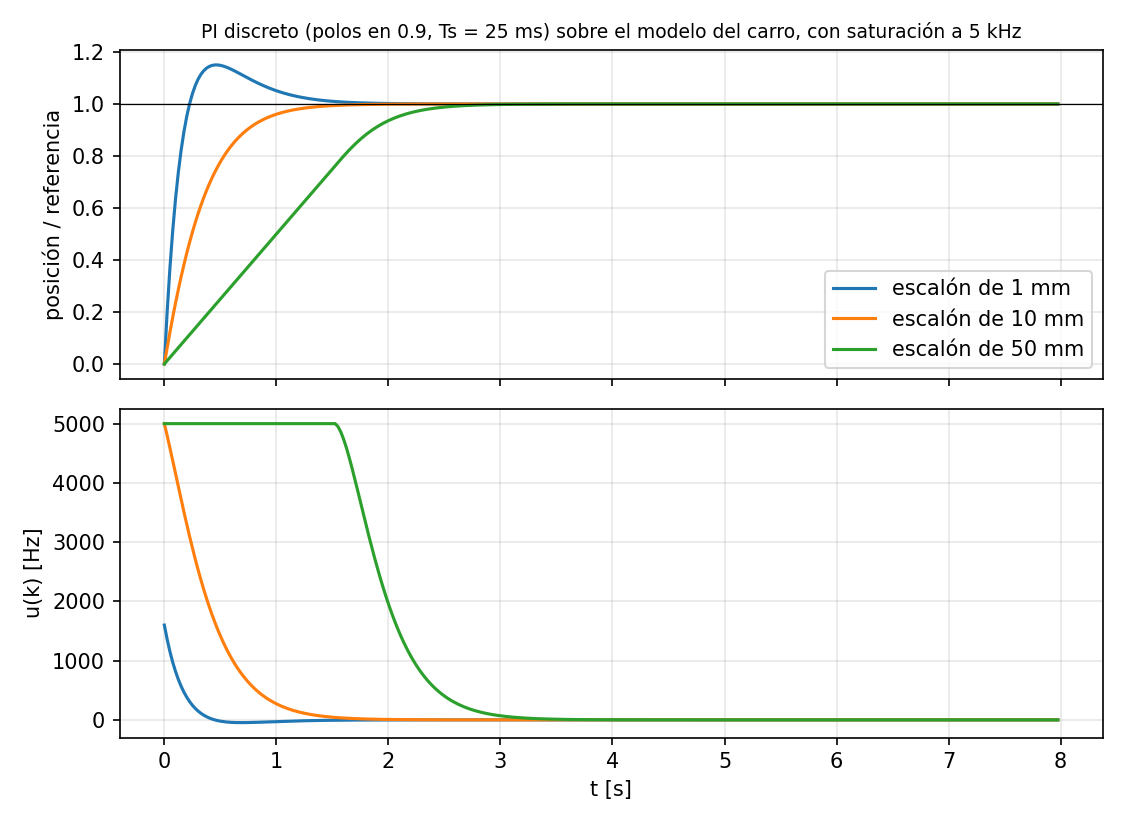
\includegraphics[width=0.72\linewidth]{../lab06_control_discreto_y_middleware/pi_respuesta_simulada.png}
\caption{PI discreto sobre el modelo del carro (\textbf{simulación}).}
\end{figure}
El sobreimpulso en escalones pequeños lo produce el cero del PI; el LQR del laboratorio 7 no lo tiene.

\subsection{Rutina de interrupción y prueba de lazo flotante}
\codigo{gemelo-digital/plc/pi\_lazo\_flotante.awl} implementa la ecuación en la interrupción temporizada 0: \codigo{SMB34 = 25} (25~ms), \codigo{ATCH INT0, 10}, aritmética REAL, saturación a $\pm$5000~Hz con el valor saturado guardado como $u(k-1)$ (antiwindup), $e(k-1)$ y $u(k-1)$ en \codigo{VD1312} y \codigo{VD1320}, y la salida libre Q1.0 que cambia en cada interrupción para medir $T_s$ y el jitter con el osciloscopio. La acción $u(k)$ \textbf{no} se envía al tren de pulsos: solo se publica en \codigo{VD1316}.

La prueba de lazo flotante (\codigo{pi\_discreto.py flotante}) ejecuta la rutina paso a paso (modo 1: la PC pide un paso con un error simulado y lee $u(k)$) con 60 pasos de escalones y rampa, y compara cada $u(k)$ del PLC con la ecuación. Contra el emulador de la rutina (REAL de 32 bits) la diferencia máxima es 0~Hz (\codigo{lazo\_flotante\_EMULADO.csv}).
\aviso{La rutina \textbf{no se cargó ni probó en el PLC}. Antes de la entrega: importarla en \codigo{brazo\_gemelo.mwp}, con los drivers desenergizados correr \codigo{pi\_discreto.py flotante --puerto COMx} y medir Q1.0 con el osciloscopio. Cerrar el lazo de verdad sigue requiriendo un sensor de posición.}

\section{ETN-1034: escalado y lógica de eventos discretos}
\subsection{Escalado a unidades de ingeniería}
Los registros del PLC están en pulsos. El middleware los convierte con las constantes de calibración:
\begin{center}\small
\begin{tabular}{l c c l}
\toprule
\textbf{Eje} & \textbf{Registro} & \textbf{Constante} & \textbf{Unidad}\\
\midrule
base & pulsos contados & 190,3 pulsos/° (medido) & grados\\
carro X & pulsos contados & 200 pulsos/mm (SUPUESTO husillo 5~mm) & mm\\
carro Y & pulsos contados & 200 pulsos/mm (SUPUESTO husillo 5~mm) & mm\\
\bottomrule
\end{tabular}
\end{center}
El brazo no tiene entradas analógicas (no hay módulo EM 231), así que no hay escalado de cuentas del ADC.

\subsection{Supervisión por eventos y parada}
El programa \codigo{brazo\_gemelo} corta los trenes de pulsos de forma determinista ante:
\begin{itemize}
\item el pulsador de paro (I0.6) o el selector en manual (I0.5 = 0);
\item un final de carrera en la dirección del movimiento;
\item el \textbf{watchdog}: con una orden de la PC en curso, el latido \codigo{VW1102} debe cambiar cada 2~s; si la PC deja de responder, el PLC detiene el movimiento (error 3);
\item una orden fuera de recorrido o sin homing, que se rechaza antes de mover.
\end{itemize}
La secuencia de homing, que coordina los ejes con estos eventos, está modelada como red de Petri en el manual técnico (capítulo 7).

\section{ETN-1000: middleware de telemetría}
\subsection{Lectura cíclica del PLC}
El middleware está en Python sin dependencias (\codigo{gemelo-digital/app/}). En lugar de Node-RED y Modbus, usa el protocolo nativo del S7-200, \textbf{PPI}, por el puerto 0 RS-485 a 9600~bit/s (manual técnico, capítulo 9):
\begin{itemize}
\item lee en cada ciclo las entradas, salidas y la zona de memoria del programa (órdenes y estado, a partir de \codigo{VB1100});
\item espera una pausa de 150 bits antes de cada trama, sin la cual el PLC ignoraba las tramas seguidas;
\item cada lectura completa tarda unos 155~ms (medido con la planta).
\end{itemize}

\subsection{Empaquetado JSON}
El estado se publica como objeto JSON en \codigo{GET /api/estado}. Ejemplo de la estructura (campos principales):
\begin{lstlisting}[basicstyle=\ttfamily\scriptsize]
{"conectado": true, "perfil": "gemelo",
 "theta_deg": 0.0, "sX_mm": 85.0, "sY_mm": 85.0,
 "entradas": {"I0.0": false, "I0.1": false, ..., "I0.5": true},
 "salidas":  {"Q0.0": false, ..., "Q0.7": false},
 "mando": true, "mando_de": "operador1"}
\end{lstlisting}

\subsection{Inserción en PostgreSQL: \codigo{telemetria.py}}
El registrador corre en un hilo aparte de la lectura del PLC: toma el último estado una vez por segundo, así una base lenta o caída no frena la lectura PPI ni el watchdog. Usa \codigo{psycopg} con sentencias parametrizadas (ningún dato se pega en el texto SQL) y guarda:
\begin{itemize}
\item \codigo{ciclo\_operacion}: uno por cada modo elegido, con su programa del PLC; al conectar cierra los ciclos que quedaron abiertos por un cierre inesperado;
\item \codigo{muestra}: una muestra por segundo de ZI-101, ZI-102, ZI-103 (PV) y SY-100, SY-101 (MV, frecuencia de cada tren mientras está activo);
\item \codigo{estado\_io}: cada cambio de las 22 señales; \codigo{evento\_alarma}: errores del PLC (watchdog, paro, fuera de recorrido, sin homing, ocupado) y pérdida de comunicación, con su despeje;
\item \codigo{orden} y \codigo{orden\_parametro}: cada orden con quién la dio, si se aceptó y el motivo del rechazo; \codigo{sesion}: cada ingreso, exitoso o fallido.
\end{itemize}
Además escribe siempre un CSV por sesión en \codigo{app/telemetria/}, con o sin base. Si no hay PostgreSQL la app funciona igual y reintenta cada 30~s.
\begin{lstlisting}[style=sql]
INSERT INTO muestra (ciclo_id, variable_id, instante, valor) VALUES (%s, %s, %s, %s)
\end{lstlisting}

\paragraph{Auditoría de inserción (tarea 39).} Prueba con el PLC simulado sobre una base de prueba (\codigo{brazo4gdl\_prueba}, 18/11/2026): 3360 muestras, \textbf{ninguna duplicada} (clave ciclo--variable--instante), periodo entre muestras de 1,000~s (mínimo 0,998, máximo 1,002), 122 cambios de señales y 23 órdenes registradas. El trigger del laboratorio 5 sigue activo: una muestra fuera de rango no se guarda y deja la alarma.

\subsection{Latencia y carga sobre el PLC}
El PLC tiene un solo maestro PPI (la app) y la tasa de lectura está limitada por el protocolo, no por la app: unos 6 ciclos por segundo. Los clientes web no consultan al PLC; leen el último estado guardado por la app. Así, aunque haya varios navegadores conectados, el PLC recibe siempre la misma carga.

\section{Entregables (Definition of Done)}
\begin{dod}
Código del PLC (.mwp) con interrupción y ecuación de diferencias & \parcial & \codigo{brazo\_gemelo.mwp} (posicionamiento y watchdog) y \codigo{pi\_lazo\_flotante.awl} (PI por interrupción, SMB34 = 25~ms); falta cargarlo y probarlo en el PLC\\
Flujo del middleware (Python) con JSON e inserción en PostgreSQL & \cumple & \codigo{brazo.py} (PPI), \codigo{gemelo\_brazo.py} (JSON) y \codigo{telemetria.py} (PostgreSQL); inserción probada con el PLC simulado, falta una corrida con la planta\\
Bitácora lazo abierto frente a lazo cerrado & \falta & no hay lazo cerrado (sin sensor de posición)\\
\end{dod}

\section{Pendientes antes de la entrega}
\begin{enumerate}
\item Instalar PostgreSQL y \codigo{psycopg} en la PC del laboratorio, crear la base y operar el brazo una sesión con la telemetría activa.
\item Cargar \codigo{pi\_lazo\_flotante.awl}, correr la prueba de lazo flotante contra el PLC con los drivers desenergizados y medir Q1.0 con el osciloscopio (periodo y jitter).
\item Para cerrar el lazo: sensor de posición (encoder leído con HSC); sin él, la bitácora lazo abierto frente a lazo cerrado solo puede ser simulada.
\end{enumerate}

\end{document}
